%! TEX root = ../main.tex
\documentclass[main]{subfiles}

\begin{document}

\chapter{論文の構成}

\section{表紙・裏表紙}
表紙には図~\ref{fig1} に示す内容を中央揃えで書く.
受領印が押されるので誤字脱字がないよう万全を期す.
裏表紙には何も印刷しない.

\begin{figure}[p] % 図は必ず[p]で取り込むこと
\begin{center}
    \includegraphics[scale=1.0]{figures/coverpage.eps}
\caption{修士論文・卒業研究報告書の表紙の例}
\label{fig1} % \label は \caption の直後に付ける
\end{center}
\end{figure}

\section{和文概要}
概要は,背景,目的,方法,結果,結論を簡潔明快に1ページ以内で記述する.
本文中に説明のある特定の記号,数式,図表などを引用しない.
図表は含めない.

% textlint-disable no-doubled-joshi,sentence-length
卒業研究報告書では,1行目に[研究題目],3行目に
[平成○○年○月○日(提出日)][学生番号][氏名],5行目に「概要」と書き,
6行目から概要を書く.
% textlint-enable no-doubled-joshi,sentence-length

修士論文の場合,学務課に提出する「様式2号学位論文の要旨(和文)」のコピーを
付せばよい.
全項目記入済みの様式2を別途印刷して付してもよいが,学務課に提出するものと
修士論文に付すものの記載内容が異ならないように注意すること.
修士論文に付す和文概要には押印の必要はないが,押印されていても印影のコピーが
あっても差し支えはない.

\section{英文概要(修士論文のみ)}
学務課に提出する「Form 2」のコピーを付す.

\section{目次}
1行目に「目次」と書き,3行目から本文の章・節毎に該当ページを列挙する.
謝辞,付録についても該当ページを列挙する.本文中に用いる記号をまとめて
説明・定義するページを作る場合は目次の直後につける.

\section{本文+図表}
第1章緒言から第n章結言までと,参考文献,謝辞を本文とし,それより後ろは
付録とする.
図表は独立した1ページとして扱い,本文で最初に言及したページの直後に
挿入する.
2, 3の図表を1ページに収めてもよい.
参考文献は,本文中の適当な箇所に半角で[12]等の番号を付けて引用する.
上付きにはしない.
章を改めるときは改ページするが,章を奇数ページから始める必要はない.

以下,本文のどこに何を書くのかを順に説明する.

\begin{description}
\item[1. 緒言(序論,はじめに)]  \\*
本研究の目的(何をどこまで明らかにするのか),研究分野における位置付け,
意義,歴史的背景,先行研究の概要などを説明し,第2章以下の構成(どの章で
何を述べるか)を列挙する.
概要とは異なり,緒言は単独では読まないので,本文中の図,式,文字,記号
等を引用してもよい.
\item[2. 第2章から第(n-1)章]  \\*
研究方法,研究結果を読者が理解しやすいように章分けし,固有の章見出しを
つける.
各章は,さらに節に細分し,固有の節見出しをつける.
章・節の番号付けは2.(ピリオドをつける), 2.1,2.1.1のようにする.
\item[3. 第n章結言(結論,まとめ)]  \\*
概要は本文全体を要約するが,結言は研究方法と研究結果のみを要約し,
緒言は含めない.
自説と比較のため第2〜(n-1)章に掲載した先行研究や従来手法なども含めない.
達成したことをまとめるのが目的なので,積み残したこと(今後の課題)は
簡潔に書く.
\item[4. 謝辞]  \\*
結言に続いて行を改め(改ページはしない),ご指導頂いた方々,便宜を図って
頂いた方々や組織(研究助成等で指導教員から記載するよう指示がある場合)に
謝辞を述べる.
相手に失礼のないよう,氏名はフルネームで書き,所属や肩書きなども
正確に書く.
データや試料のご提供など,特定の事項については脚注に記してもよい.
\item[5. 参考文献]  \\*
参考文献の書誌情報を,本文で引用した順に箇条書きする.
書き方を以下に引用
する\footnote{電子情報通信学会和文論文誌投稿のしおり(情報・システム
ソサイエティ) 2.6.1文献のリスト法より引用.}.
\begin{itemize}
\item[(a)] 付録Gの「学術雑誌略語表」
	   \footnote{http://www.ieice.org/jpn/shiori/pdf/furoku\_g.pdf}
	   に掲載されている雑誌名は,同表に従って略語で記す.
\item[(b)] 著者が複数の場合には,全著者の氏名を記入する.なお,欧文の場
	   合にはイニシャルと姓名を記入し, A.G. Wine のようにイニシャル
	   と姓の間にのみ半角スペースを挿入する.
\item[(c)] 英文論文の標題中の単語については,文頭以外は小文字を使用する.
\item[(d)] 欧文文献においては,常に半角ピリオド「.」と半角カンマ「,」を
	   用いる.和文文献においては,読点には全角の「,」を用い,
	   「vol.」,「no.」,「pp.」あるいは月名等の省略記号及び行末の
	   句点には半角ピリオド「.」を用いる.なお,vol.J62-B,no.1,
	   pp.20-27等の場合には,半角ピリオド「.」の後ろにはスペースは挿
	   入しない.
\item[(e)] 発行の年月を記載する場合には,月年の順で,月名には英語を,年
	   には西暦を用いる.
\item[(f)] WebページのURLの参照は,新規性,有効性,信頼性の明確化,ある
	   いは論旨の補強など,必要に応じて効果的に使う.ただし,第三者
	   のWebページは改版や消滅などの可能性が高いので,できるだけ原著
	   を参照する.
\end{itemize}
表~\ref{tab2} に,文献種類毎に整理した参考文献の書式を示す.
\end{description}

\begin{table}[p]
\begin{center}
\caption{参考文献の書式}
\label{tab2}
\begin{tabular}{p{36mm}|p{105mm}} \Hline
文献種類 & 書誌情報の書式 \\ \hline
雑誌\cite{YY79}\cite{RWG64}
 & 著者名,``標題,'' 雑誌名,巻,号,pp.を付けて始め−終りのページ,月年. \\ \hline
著書,編書\cite{Y89}\cite{TON90}
 & 著者名,書名,編者名,発行所,発行都
市名,発行年. \\ \hline
著書の一部を引用する場合\cite{YA89}\cite{HSR72}
 & 著者名,``標題,'' 書名,編者名,章番号またはpp.を付けて始め−終り
のページ,発行所,発行都市名,発行年.\\ \hline
国際会議\cite{YMI90}
 & 著者名,``標題,'' 会議名,no.を付けて論文番号,
   pp.を付けて始め−終りのページ,開催都市名,国名,月年. \\ \hline
国内大会,研究会論文集\cite{KK95}
 & 著者名,``標題,'' 学会論文集名,分冊または号,
   no.を付けて論文番号,pp.を付けて始め−終りのページ,月年.\\\hline
電子媒体\cite{KK79}
 & 著者名,``標題,'' 雑誌名,巻,号,pp.を付けて始め−終りのページ,
   月年(オンライン),入手先 $\langle$ 参照例$\rangle$ ,(参照日付)
   \\\hline
Webページ\cite{ieice}
 & 著者名,Webページタイトル,Webサイト名(オンライン), 
   入手先$\langle$ 参照例$\rangle$ (参照日付).\\\Hline
\end{tabular}
\end{center}
\end{table}



\section{付録}
以下の内容は本文に書かず付録として本文の後ろにまとめて書く.

\begin{itemize}
\item 本文中の数式の誘導が複雑で,論旨に直接関係ないとき.
\item 引用した文献の内容を詳しく説明したいとき.
\item 実験の詳細なデータを本文中に収めると,本文の構成が複雑になるとき.
\end{itemize}

付録はページを改めて書き,項目毎に,「付録A. ○○」のように表題を付す.
付録は通読されるべきものに限定すること.
ソースコードやデータのダンプリスト等,常識的に通読しないものは,本文
にも付録にも含めてはならない.

\end{document}

